\documentclass[tikz]{standalone}
\usepackage{tikz}

\begin{document}
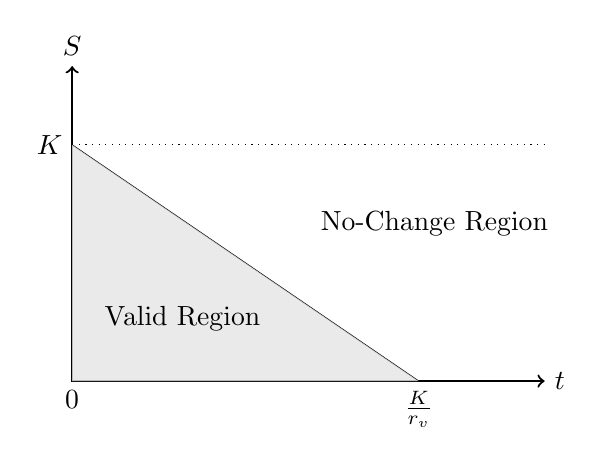
\begin{tikzpicture}[scale=2.0]
	\coordinate[label=below:{$0$}] (origin) at (0,0);
	\draw[<->, thick] (0,2) node (saxis) [above] {$S$}
	|- (3,0) node (taxis) [right] {$t$};
	
	\coordinate[label=left:{$K$}] (sintercept) at (0,1.5);
	\coordinate[label=below:{$\frac{K}{r_v}$}] (tintercept) at (2.2,0);
	\draw (sintercept) -- (tintercept);
	\fill[gray!20, opacity=0.8] (origin) -- (sintercept) -- (tintercept) -- cycle;

	\draw[dotted] (sintercept) -- (3.0, 1.5);
	\node (valid) at (0.7,0.4) {Valid Region};
	\node (endregion) at (2.3, 1.0) {No-Change Region};
\end{tikzpicture}
\end{document}
